% GFA specifications
\chapter{Le specifiche GFA}

In questo capitolo verrà fornita un'ampia panoramica sulle specifiche
GFA, sulle linee presenti e sulle diverse circostanze di assemblaggio
di sequenze che possono essere rappresentate.
Verrà inoltre fornita una breve introduzione ad alcuni concetti
biologici riguardanti gli elementi che compongono DNA e RNA e
la loro struttura, necessarie a comprendere le diverse situazioni
descritte nelle specifiche.

\section{Introduzione a GFA, motivazioni e struttura}
GFA è l'acronimo per Graph Assembly Format, è un
formato per la rappresentazione dei legami presenti fra le sequenze di
un genoma al fine di riuscire a ricostruirne la struttura.
Le motivazioni che risiedono alla base della proposta per un nuovo
formato consistono nell'uniformare le notazioni che programmi
di visualizzazione, di assemblaggio e di manipolazione potessero
utilizzare.

La prima versione della specifica GFA viene indicata col termine
GFA1. Questa prima versione, come vedremo successivamente,
limita la descrizione delle possibili situazioni in cui due sequenze
possono trovarsi in relazione. Per questo motivo, e per estendere
maggiormente l'insieme delle informazioni utili da descrivere,
è stata sviluppata una seconda specifica, indicata con GFA2.
Questa specifica generalizza, usando un'unica notazione,
i collegamenti fra sequenze descritti da GFA1 e permette inoltre
di descrivere relazioni di ogni tipo fra due sequenze.
GFA2 è un \emph{superset} di GFA1 e come tale permette
(con un minimo numero di operazioni) di trasformare un file GFA2
nell'analogo (rappresentabile) in GFA1. Questa seconda specifica
è stata appositamente pensata per permettere la descrizione di
sequenze e collegamenti imponendo un minimo numero di vincoli,
permettendo all'utilizzatore di impiegarla per la descrizione di dati
indipendentemente dai dettagli che questi forniscono.

Entrambe le specifiche adoperano la stessa formattazione delle linee.
Una linea descrive un'informazione di assemblaggio, sia
essa una sequenza, un collegamento o un insieme di elementi.
In ogni riga, il primo carattere indica
l'identità della linea stessa alla quale seguono, separati esclusivamente
da tabulazioni, gli elementi che costituiscono l'informazione
che la linea descrive e che prendono il nome di \emph{campi}.
I campi possono essere definiti o meno, nel qual caso l'assenza
dell'informazione viene indicata con un asterisco \texttt{*}.

In ogni linea di entrambe le specifiche è possibile descrivere campi
opzionali (che possono essere predefiniti per una linea o introdotti
direttamente dall'utente), descritti nel formato \texttt{TAG:TIPO:CONTENUTO}
dove \texttt{TAG} è una sequenza di due caratteri alfanumerici
(in maiuscolo se il campo è predefinito dalla linea, in minuscolo
altrimenti) che identifica l'informazione che esso indica.
Il \texttt{TIPO} di un campo viene anch'esso descritto da un
identificatore, ciascuno indicante il seguente contenuto:

\noindent
\begin{table}[h]
	\rowcolors{1}{white}{lightgray}
	\begin{tabularx}{\textwidth}{ | X | l | }
		\hline
		Tipo	&	Descrizione\\
		A 		&	Singolo carattere stampabile(escluso lo spazio)\\
		i 		&	Intero con segno\\
		f 		&	Decimale con precisione singola\\
		Z		&	Stringa stampabile (incluso lo spazio)\\
		J		&	Stringa JSON, escludendo caratteri di newline e di tabulazione\\
		H 		&	Array di Byte in formato esadecimale\\
		B 		&	Array di interi o di decimali\\
		\hline
	\end{tabularx}
	\caption{Tabella dei tipi che è possibile usare per specificare campi opzionali.}
	\label{tab:optfield-type}
\end{table}

\begin{wrapfigure} {O} {0.65\textwidth}
        \begin{centering}
                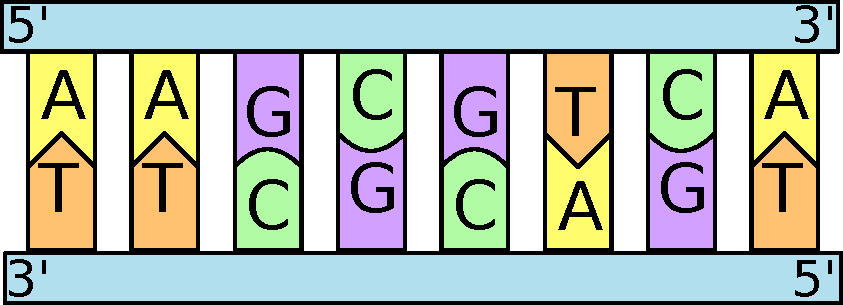
\includegraphics[scale=0.5]{dna-strand}
                \caption[Rappresentazione del DNA]{Rappresentazione grafica degli strand che compongono il DNA.}
                \label{fig:dna-strand}
        \end{centering}
\end{wrapfigure}

Mentre verranno analizzate le linee delle due specifiche, è essenziale
avere un'idea di cosa sia una sequenza e di come questa può essere in
relazione con le altre.
Con il termine sequenza viene indicata una \emph{sequenza nucleotidica},
un susseguirsi di lettere che denotano le unità molecolari che compongono
gli acidi nucleici di RNA e DNA (\emph{nucleotide}).
Una sequenza è priva di un ordine specifico, ma è possibile attribuirgliene
uno osservando la composizione del tipo di legame che collegano
gli elementi costitutivi il nucleotide, in base all'orientamento del
legame presente tra le unità di carbonio 3' di un un'unità
e la stessa unità 5' della successiva. Grazie a tale osservazione
è possibile individuare un ordinamento che verrà definito
come 5'3'.

Oltre questa considerazione, bisogna tenere conto che
l'informazione presente nel DNA
è la stessa a parità di estremità, ma in ordine inverso e
complementato (vedi figura \ref{fig:dna-strand}) (sostituendo
la citosina con la guanina e
l'adenina con la timina). Nel caso di RNA alla timina
si sostituisce l'uracile, ma il processo di formazione del RNA
prevede anch'esso questa operazione di complementazione
della sequenza.

Ergo, quando si considera una sequenza (nel caso
dell'assemblaggio del DNA), è necessario tenere presente
che un collegamento fra due sequenze potrebbe considerare
una sequenza posta sullo strand (una delle estremità
che compone l'elica del DNA) opposto e di conseguenza una loro
sovrapposizione potrebbe richiedere un preprocessamento della
stringa che la porti ad essere coerente con l'altra, operazione
che prende il nome di \emph{reverse and complement}.

% GFA1
\section{Linee GFA1}
GFA1 è la prima versione della specifica, essa si concentra nella descrizione
delle sequenze, collegate tra loro da una relazione di \emph{contenimento}
o di \emph{successione}.

Le linee previste dalla specifica sono header, segment, link, containment
e path.

L'header è una riga il cui scopo è quello di indicare la versione della specifica
in uso, può ripresentarsi più volte all'interno del file per indicare parametri
opzionali validi per tutti gli elementi. Tale linea viene indicata con il simbolo \texttt{H}.

\subsection{Segment}
La linea di Segment (indicata con il simbolo \texttt{S}) descrive in termini
generici una sequenza, la quale può essere definita o no. All'informazione
viene attribuito un identificativo che deve essere unico in tutto in file.
A queste proprietà se ne possono aggiungere altre, descritte da campi
opzionali, tra i quali la lunghezza (\texttt{LN}) e
il conto dei \emph{k-meri} (l'insieme di tutte le possibili sottostringhe
di lunghezza k contenute nella stringa).

\begin{lstlisting}[basicstyle=\ttfamily, caption=Una possibile Segment line.]
S	5	CCCGGGGTAA		LN:i:10
\end{lstlisting}

\subsection{Link}
\label{sec:link}
I Link (indicati dal simbolo \texttt{L}) sono il principale
tipo di relazione fra due sequenze. Essi
indicano una sovrapposizione fra le sequenze indicate da due Segment.
Nello specifico, un Link fra due Segment indica che la parte terminale
della prima sequenza è coinvolta in una sovrapposizione (\emph{overlap})
con l'inizio della seconda; il termine che descrive esattamente questa situazione
è \emph{dovetail overlap}. Tale tipologia di collegamento costituisce
un'informazione di rilievo nell'analisi dell'assemblaggio poiché descrive
un susseguirsi fra due sequenze.

Il link non solo descrive questa situazione, ma indica anche quale
estremità della sequenza è coinvolta nel overlap. Ricordando che
l'informazione contenuta nella struttura elicoidale del DNA è la stessa a parità
di estremi (ma in senso inverso e complementata), è possibile
che due sequenze siano contigue (in una situazione di dovetail
overlap) considerando la loro provenienza da due estremità
diverse dell'elica (strand).
Il link permette di esprimere il collegamento considerando anche questa
particolarità; per farlo esso utilizza un segno ``\texttt{+}'' per indicare
che la sequenza non necessita di alcun processamento nel suo
coinvolgimento nella sovrapposizione, mentre utilizza un segno ``\texttt{-}''
per esplicare la necessità di effettuare un' operazione di reverse
and complement sulla sequenza prima di poterla considerare
nel overlap.

Visto che, come dicevo poc'anzi, un Link descrive una sovrapposizione
tra la fine della prima sequenza e l'inizio della seconda (indipendentemente
dai segni associati alle due sequenze coinvolte), ciò da luogo a quattro
possibili situazioni:
\begin{itemize}
	\item la parte destra della prima sequenza si sovrappone con la parte
		sinistra della seconda (vedi figura \ref{fig:dov-ov}\subref{fig:dov-ov++});
	\item la parte destra della prima sequenza si sovrappone con la parte
		destra della seconda (vedi figura \ref{fig:dov-ov}\subref{fig:dov-ov+-});
	\item la parte sinistra della prima sequenza si sovrappone con la parte
		sinistra della seconda (vedi figura \ref{fig:dov-ov}\subref{fig:dov-ov-+});
	\item la parte sinistra della prima sequenza si sovrappone con la parte
		destra della seconda (vedi figura \ref{fig:dov-ov}\subref{fig:dov-ov--}).
\end{itemize}

\captionsetup{justification=centering}
\begin{figure}[h]
	\begin{subfigure}{.5\linewidth}
	  \centering
	  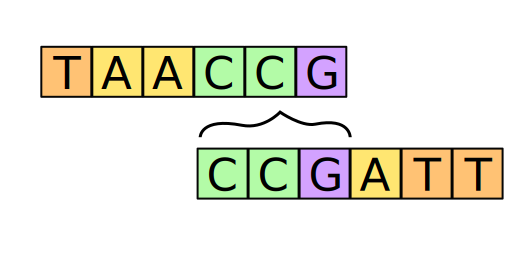
\includegraphics[scale=0.4]{dov_ov_++}
	  \caption{}
	  \label{fig:dov-ov++}
	\end{subfigure}%
	\begin{subfigure}{.5\linewidth}
	  \centering
	  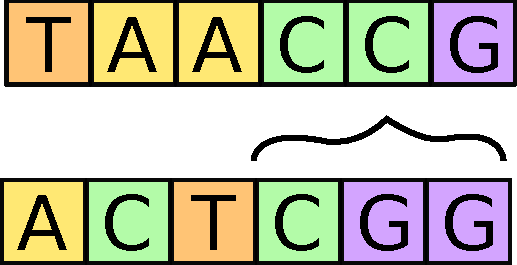
\includegraphics[scale=0.4]{dov_ov_+-}
	  \caption{}
	  \label{fig:dov-ov+-}
	\end{subfigure}%
	
	\bigskip%
	
	\begin{subfigure}{0.5\linewidth}
	  \centering
	  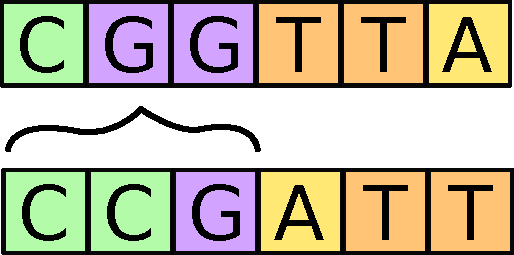
\includegraphics[scale=0.4]{dov_ov_-+}
	  \caption{}
	  \label{fig:dov-ov-+}
	\end{subfigure}%
	\begin{subfigure}{0.5\linewidth}
	  \centering
	  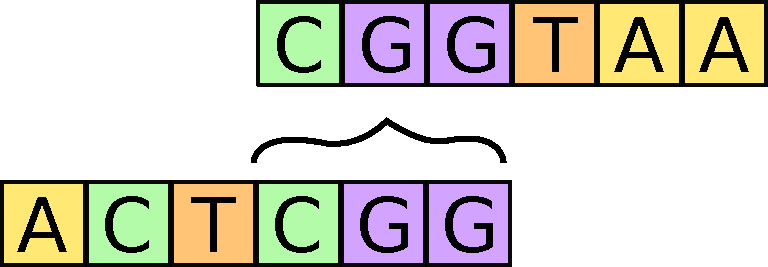
\includegraphics[scale=0.4]{dov_ov_--}
	  \caption{}
	  \label{fig:dov-ov--}
	\end{subfigure}
	
	\captionsetup{justification=justified}
	\caption[Rappresentazione delle possibili situazioni di dovetail overlap]{
		\textit{(a)} Dovetail overlap senza bisogno di alterare le sequenze.
		\textit{(b)}  Dovetail overlap dove la seconda sequenza necessita
	  		di un'operazione di reverse and complement per sovrapporsi alla prima.
	  	\textit{(c)} Un'operazione di reverse and complement deve essere eseguita
	  		sulla prima sequenza, affinché ci sia un overlap.
	  	\textit{(d)} Entrambe le sequenze richiedono operazioni di reverse and complement.}
	\label{fig:dov-ov}
\end{figure}
\captionsetup{justification=justified}

Oltre a questa considerazione sulle sequenze, il Link fornisce una descrizione
dell'allineamento, dato da una stringa CIGAR. Una stringa CIGAR è
una serie di lettere e numeri che descrivono lo stato di somiglianza
fra le due sequenze.
Tra i campi opzionali che il Link predispone si trova il campo
\texttt{ID}, mediante il quale è possibile riferirsi a tale
linea.
\clearpage

\subsection{Containment}
\label{sec:containment}
\begin{wrapfigure} {O} {0.35\textwidth}
	\begin{centering}	
		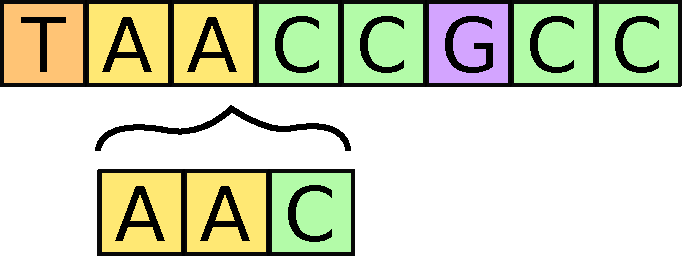
\includegraphics[scale=0.35]{containment}
		\caption[Rappresentazione di una situazione di contenimento fra sequenze]
		{Una rappresentazione grafica della situazione di contenimento fra due sequenze.}
		\label{fig:containment}
	\end{centering}
\end{wrapfigure}
Le linee di Containment (indicate con il simbolo \texttt{C})
descrivono sovrapposizioni fra sequenze nelle quali una stringa intera
è contenuta nell'altra.
I campi descrivono le stesse informazioni dei Link, ma è bene notare
i dettagli circa le posizioni delle sequenze che una sovrapposizione di
questo tipo comporta.
Date due sequenze $s1$ ed $s2$, un Containment tra la sequenza $s1$ e la
sequenza $s2$ indica che la sequenza $s1$ \emph{contiene} la sequenza
$s2$. In tale situazione vuole significare che la sovrapposizione comincia
dal primo carattere della sequenza di $s2$ e continua fino all'ultimo
(vedi figura \ref{fig:containment}).

Oltre ai classici campi che descrivono i nodi indicanti le sequenze coinvolte,
il loro orientamento nella sovrapposizione e l'allineamento; queste linee hanno un campo
che indica la posizione di inizio della sequenza contenuta nella sequenza
contenitrice.

\subsection{Path}
Un Path (indicato dal simbolo \texttt{P}) descrive un susseguirsi di
sequenze collegate esclusivamente da Link. Indica pertanto un percorso
all'interno del grafo di sequenze contigue. Queste linee
indicano esclusivamente gli identificativi e l'orientamento delle sequenze
coinvolte nel percorso cui seguono l'insieme delle stringhe CIGAR relative
l'allineamento delle sequenze prese a due a due.

\newpage
\captionsetup{justification=centering, singlelinecheck=false}
\begin{lstlisting}[basicstyle=\ttfamily, frame=topline, caption=Un esempio di file GFA 1.]
H	VN:Z:1.0
S	11	ACCTT
S	12	TCAAGG
S	13	CTTGATT
L	11	+	12	-	4M
L	12	-	13	+	5M
L	11	+	13	+	3M
P	14	11+,12-,13+	4M,5M
\end{lstlisting}
\captionsetup{justification=justified, singlelinecheck=false}


\section{GFA2}
GFA2 come accennato in precedenza è un'estensione di GFA1, pensata
per fornire più libertà all'utente circa le informazioni che è possibile descrivere.
Le linee appartenenti a questa specifica non comprendono campi opzionali
predefiniti, l'utente è libero di definire i campi aggiuntivi che più ritiene opportuni
per la sua applicazione.


\subsection{Segment}
Queste linee sono analoghe ai Segment in GFA1, ai campi viene aggiunto
un numero intero per descrivere la lunghezza della sequenza.
La lunghezza non vuole essere l'esatta lunghezza della sequenza, ma
vuole indicare la grandezza che tale sequenza assume quanto rappresentata
da un programma di disegno (come Bandage, descritto a pagina \pageref{sec:bandage}).
Nell'indicare le sequenze non viene più richiesto l'uso di caratteri IUPAC\cite{wiki:acid-notation},
la sequenza può essere descritta con un qualsiasi carattere stampabile,
nello specifico dal simbolo ``\texttt{!}'' al simbolo ``\texttt{\textasciitilde}''
della tabella ASCII.

\subsection{Edge}
\begin{wrapfigure} {O} {0.35\textwidth}
	\begin{centering}	
		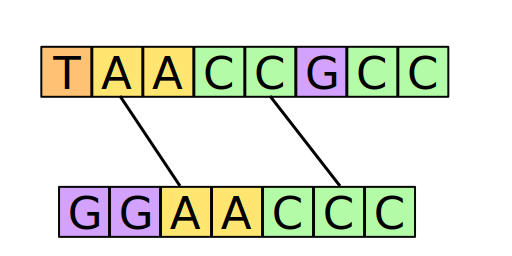
\includegraphics[scale=0.35]{generic-overlap}
		\caption[Rappresentazione di una situazione generica di sovrapposizione fra sequenze]
		{Una rappresentazione grafica di una generica di sovrapposizione fra sequenze.}
		\label{fig:generic-overlap}
	\end{centering}
\end{wrapfigure}
La linea di Edge (indicata con la lettera \texttt{E}), indica un qualsiasi
tipo di sovrapposizione. Essa quindi generalizza le linee di Link e Containment
ed aggiunge la situazione in cui una generica parte di una sequenza
è sovrapposta ad una qualsiasi parte (non solo agli estremi) di
un'altra (come rappresentato in figura \ref{fig:generic-overlap}).

Questa linea, come Link e Containment, fornisce gli identificatori
delle sequenze coinvolte nel overlap e i rispettivi orientamenti, cui
si aggiungono le \emph{posizioni} di inizio e fine delle parti
delle rispettive sequenze sulle quali si svolge la sovrapposizione.
La posizione è un intero che parte da 0 (descrivendo il primo
carattere della sequenza) e termina in posizione pari alla
lunghezza stessa della sequenza, all'ultima posizione della sequenza
si pone il simbolo ``\texttt{\$}'', non farlo costituirebbe un errore.

In questo modo si avrà che una situazione di dovetail overlap
verrà indicata da un edge in cui le posizioni delle due sequenze
sono $inizio1=0$ o $fine1 = x\$$ e $inizio2 =0$ o $fine2=y\$$;
mentre una situazione di contenimento viene descritta
da un edge in cui le posizioni delle sequenze sono $inizio1=0$ e 
$fine1=x\$$ o $inizio2=0$ e $fine2=y\$$. Si osservi che mentre
un contenimento in GFA2 non impone alcun ordine circa la sequenza
contenuta e quella contenitrice, un Containment in GFA1 prevede
che la prima sequenza sia la contenitrice e la seconda sia la contenuta;
inoltre in GFA2 non vi è alcun campo obbligatorio che indica l'inizio della
sequenza contenuta, diversamente da GFA1.

Come in GFA1 è possibile specificare l'allineamento, non solo mediante
stringa CIGAR, ma indicando una traccia DAZZLER (un indicatore
per eseguire l'allineamento fra sequenze in un tempo quasi lineare).
Quindi non solo GFA2 permette di descrivere la natura dell'allineamento tramite
CIGAR string, ma anche di descrivere un modo veloce per calcolarlo usando
le tracce DAZZLER. Come nelle altre situazioni delle specifiche, in caso
di mancata informazione viene posto un asterisco in tale campo.

Questa generalizzazione delle possibili sovrapposizioni tra due sequenze
permette di usare la specifica non solo per la descrizione di grafi di assemblaggio,
come nel caso di GFA1; ma anche di rappresentare, in un unico formato,
i risultati provenienti da diversi stadi del processo di assemblaggio.

\subsection{Fragment}
Le linee di Fragment (indicate con la lettera \texttt{F}) indicano un
collegamento fra una sequenza indicata nel file e una sequenza presente in un file esterno.
Il collegamento esprime un allineamento fra le due sequenze, in modo analogo ad
un Edge.

\subsection{Gap}
Le linee di Gap (indicate con la lettera \texttt{G}) indicano uno spazio
presente fra due sequenze, indicando la distanza che le separa e la
varianza di tale supposizione.

\subsection{Group}
I gruppi in GFA possono essere di due tipi, gli OGroup (indicati con la lettera \texttt{O})
e gli UGroup (indicati con la lettera \texttt{U}). I primi indicano una sequenza ordinata di elementi
GFA2 (escludendo gli UGroup) che individuano un percorso all'interno del grafo, mentre
gli UGroup indicano un insieme di elementi del grafo privi di ordine. Entrambi
i gruppi descrivono un sottografo che è possibile ricavare
dal grafo descritto dal file GFA.

\captionsetup{justification=centering, singlelinecheck=false}
\begin{lstlisting}[basicstyle=\ttfamily\scriptsize, frame=topline, caption=Un esempio di file GFA 2.]
S	1	122	*
S	3	29	TGCTAGCTGACTGTCGATGCTGTGTG
E	1_to_2	1+	2+	110	122$	0	12	12M
S	5	130	*
S	13	150	*
O	14	11+ 12+
S	11	140	*	xx:i:11
F	1	read1+	0	42	12	55	*	id:Z:read1_in_1
U	16	1 3 1_to_3
U	16sub	5 16
S	12	150	*
E	1_to_3	1+	3+	112	122$	0	12	10M
G	1_to_11	1+	11-	120	*
E	11_to_13	11+	13+	20	140$	0	120	120M
\end{lstlisting}
\captionsetup{justification=justified, singlelinecheck=false}

\section{Conclusioni}
In questo capitolo sono state esaminate le due versioni che costituiscono
la specifica GFA, indicando lo scopo del quale ciascuna versione intende
occuparsi e descrivendo i concetti che ciascuna linea vuole rappresentare
nel contesto dell'assemblaggio del genoma. Nel prossimo
capitolo si procederà nella descrizione del lavoro svolto nello sviluppo
di \pygfa e di come si è dovuto procedere nella rappresentazione delle
informazioni descritte nelle specifiche.